%\setprocid

% \newcommand{\TestPerfSetup}{Setup and configuration}
% \newcommand{\TestPerfRFPXA}{RF measurements with PXA}
% \newcommand{\TestPerfCCDF}{CCDF measurement}
% \newcommand{\TestPerfFreqS}{Frequency Stability}
% \newcommand{\TestPerfCWPhaseN}{Carrier Phase Noise}
% \newcommand{\TestPerfSpuriousDSN}{Spurious in DSN Band}
% \newcommand{\TestPerfFilterVector}{Data Demodulation Filter Tuning and Vector Analysis}
% \newcommand{\TestPerfBer}{Degraded link test with one X-Band channel}
% \newcommand{\TestPerfSetupBreak}{Tests setup break}

\renewcommand{\reqid}{N/A}
\renewcommand{\procid}{SB1FS-COM-P-013}
\renewcommand{\procname}{Performance Test}

\section{\procid{} \procname{}} \label{sec:SB1FS-COM-P-013}

 This section details the test procedures for EWC30 transmitter.
 The figures \ref{fig:data-setup1} and  \ref{fig:data-setup2} show the test setups.
 Solid lines are connections that apply to all downlink tests and dashed 
 lines are connections that change from one test to another.

\begin{figure}[H]\centering
	\includegraphics[width=1\linewidth]{figuras/EWC30-PXA-Setup1.png}  
	\caption{EWC30 Transmissions Test Setup}
  \label{fig:data-setup1}
\end{figure}

\begin{figure}[H]\centering
	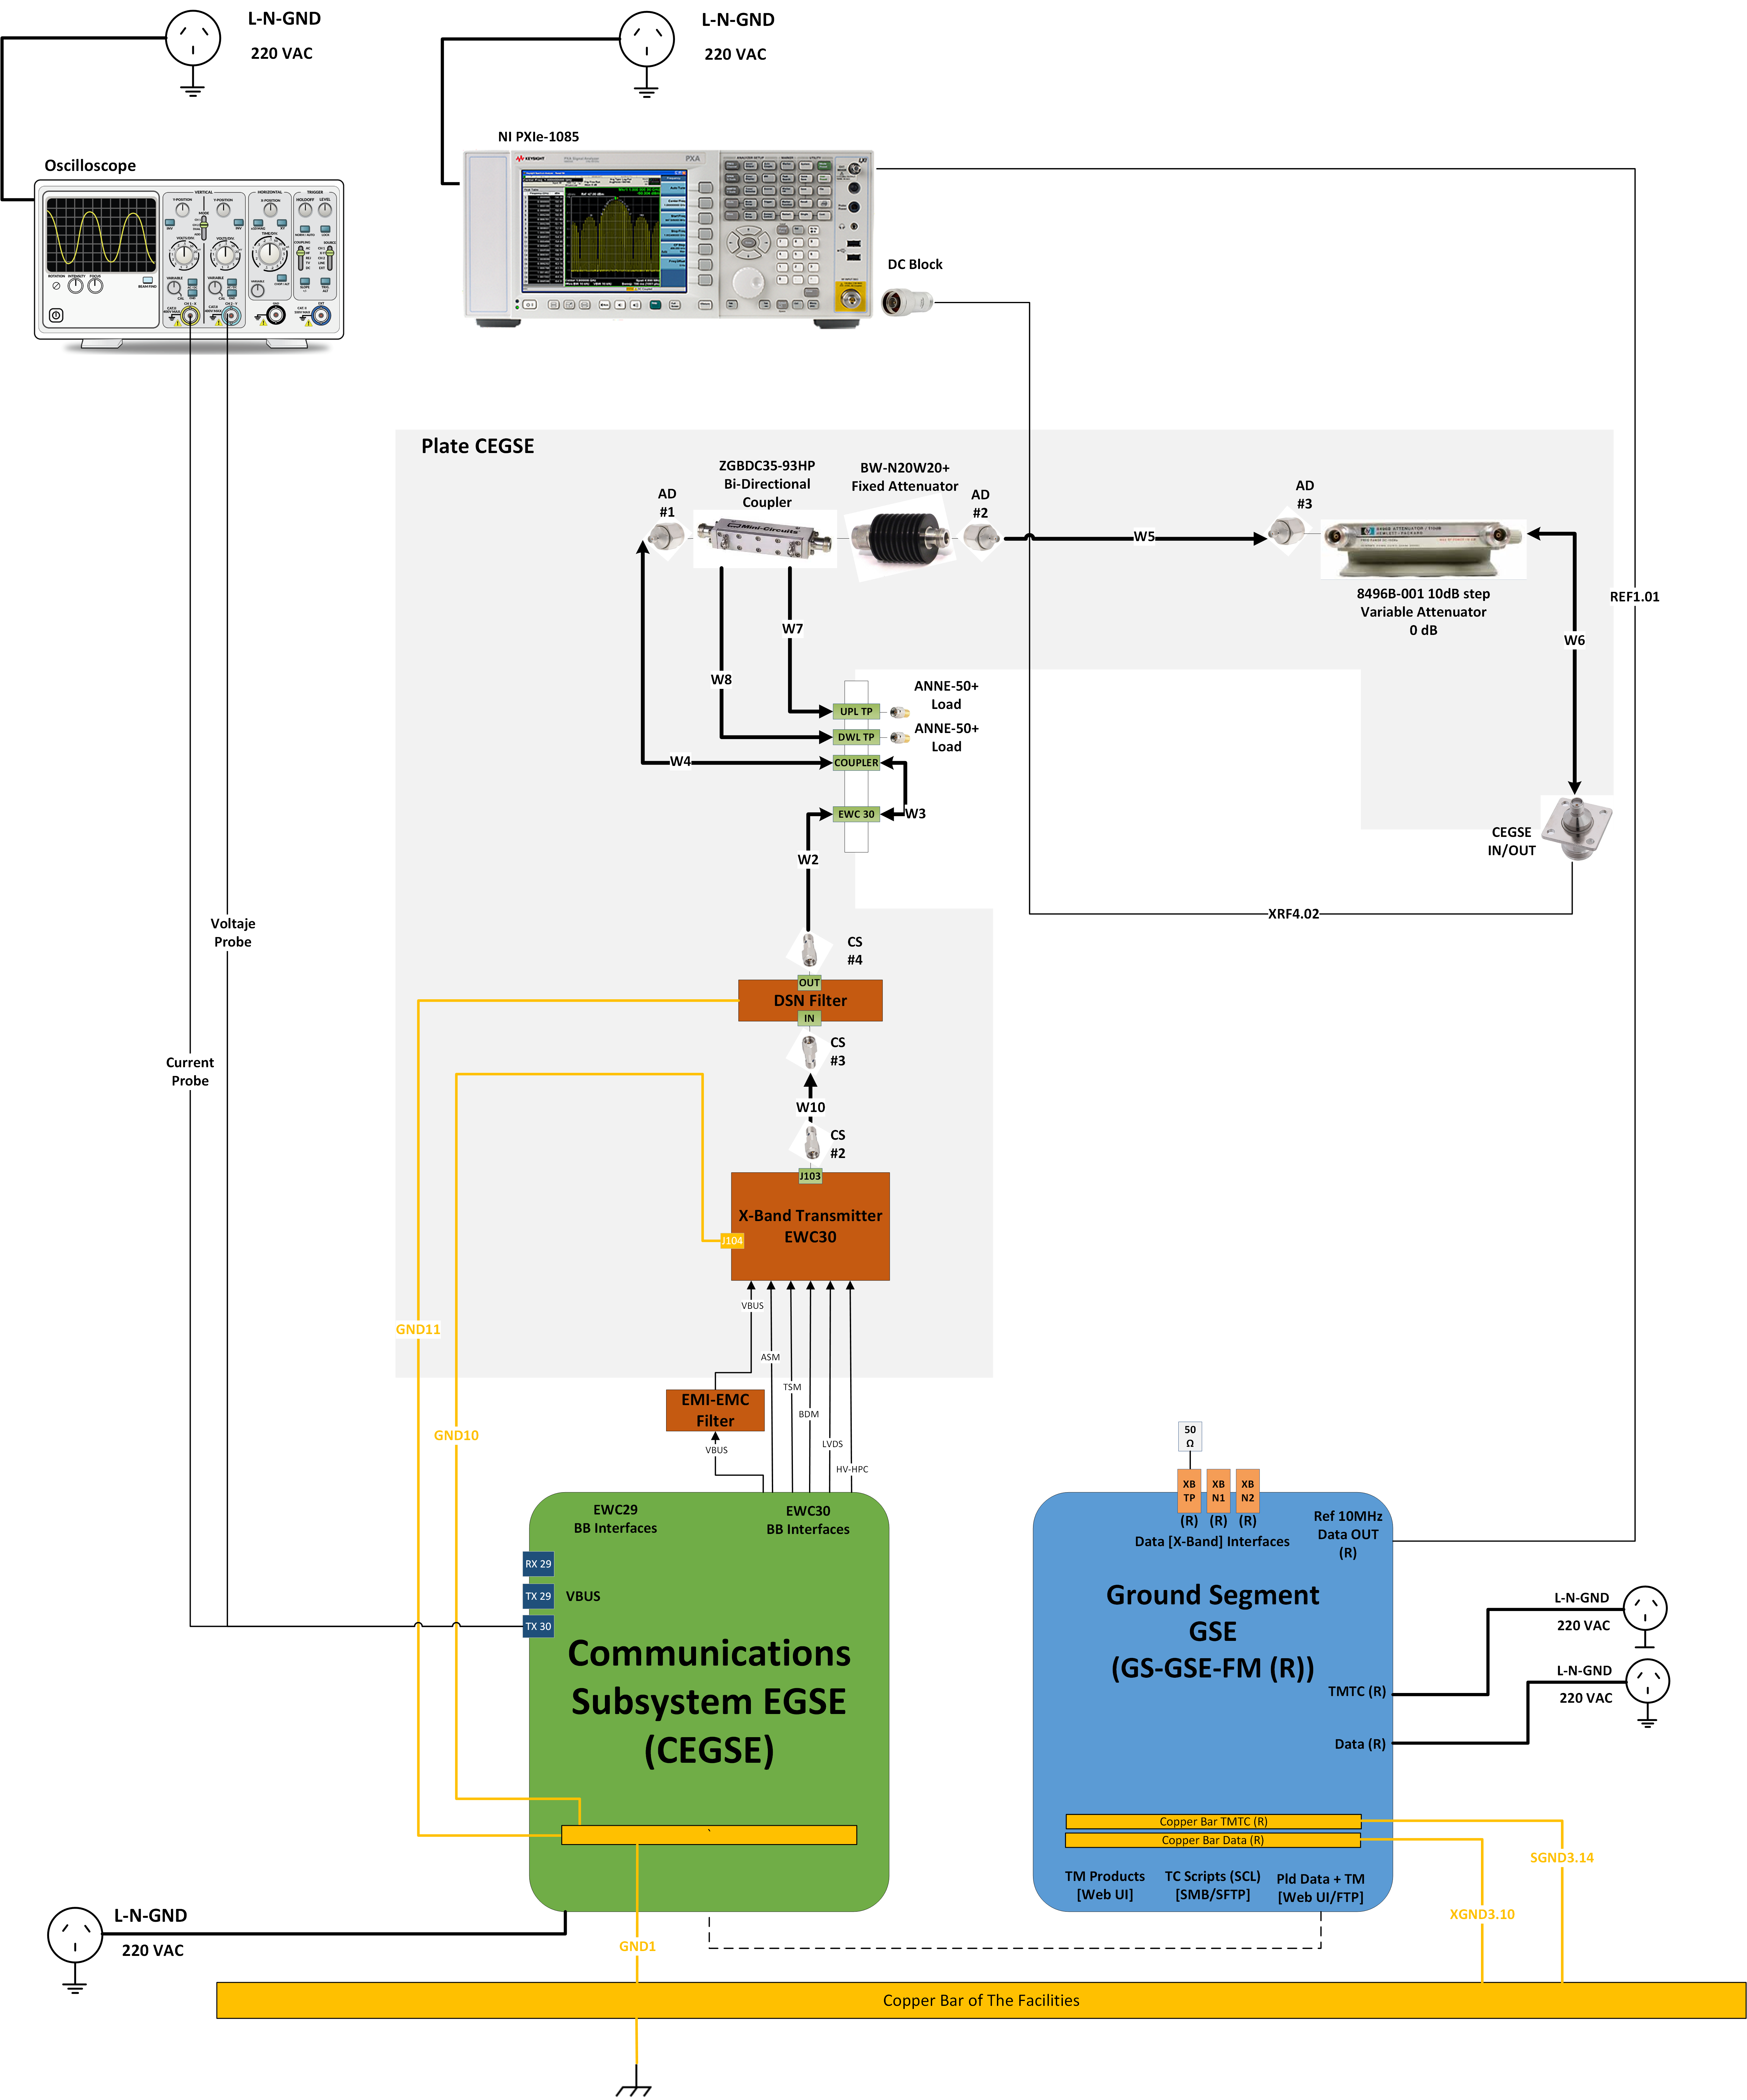
\includegraphics[width=1\linewidth]{figuras/EWC30-PXA-Setup2.png}  
	\caption{EWC30 Transmissions Test Setup (Spurious)}
  \label{fig:data-setup2}
\end{figure}
